%%%%%%%%%%%%%%%%%%%%%%%%%%%%%%%%%%%%%%%%%
% Journal Article
% LaTeX Template
% Version 1.4 (15/5/16)
%
% This template has been downloaded from:
% http://www.LaTeXTemplates.com
%
% Original author:
% Frits Wenneker (http://www.howtotex.com) with extensive modifications by
% Vel (vel@LaTeXTemplates.com)
%
% License:
% CC BY-NC-SA 3.0 (http://creativecommons.org/licenses/by-nc-sa/3.0/)
%
%%%%%%%%%%%%%%%%%%%%%%%%%%%%%%%%%%%%%%%%%

%----------------------------------------------------------------------------------------
%   PACKAGES AND OTHER DOCUMENT CONFIGURATIONS
%----------------------------------------------------------------------------------------

\documentclass[twoside,twocolumn]{article}

\usepackage{blindtext} % Package to generate dummy text throughout this template

\usepackage[sc]{mathpazo} % Use the Palatino font
\usepackage[T1]{fontenc} % Use 8-bit encoding that has 256 glyphs
\linespread{1.05} % Line spacing - Palatino needs more space between lines
\usepackage{microtype} % Slightly tweak font spacing for aesthetics

\usepackage[english]{babel} % Language hyphenation and typographical rules

\usepackage[hmarginratio=1:1,top=25mm,columnsep=25pt,textwidth=450pt]{geometry} % Document margins
\usepackage[hang, small,labelfont=bf,up,textfont=it,up]{caption} % Custom captions under/above floats in tables or figures
\usepackage{booktabs} % Horizontal rules in tables

\usepackage{lettrine} % The lettrine is the first enlarged letter at the beginning of the text

\usepackage{enumitem} % Customized lists
\setlist[itemize]{noitemsep} % Make itemize lists more compact

\usepackage{abstract} % Allows abstract customization
\renewcommand{\abstractnamefont}{\normalfont\bfseries} % Set the "Abstract" text to bold
\renewcommand{\abstracttextfont}{\normalfont\small\itshape} % Set the abstract itself to small italic text

\usepackage{titlesec} % Allows customization of titles
\renewcommand\thesection{\Roman{section}} % Roman numerals for the sections
\renewcommand\thesubsection{\roman{subsection}} % roman numerals for subsections
\titleformat{\section}[block]{\large\scshape\centering}{\thesection.}{1em}{} % Change the look of the section titles
\titleformat{\subsection}[block]{\large}{\thesubsection.}{1em}{} % Change the look of the section titles

\usepackage{fancyhdr} % Headers and footers
% \pagestyle{fancy} % All pages have headers and footers
\fancyhead{} % Blank out the default header
\fancyfoot{} % Blank out the default footer
\fancyfoot[RO,LE]{\thepage} % Custom footer text

\usepackage{titling} % Customizing the title section

\usepackage{hyperref} % For hyperlinks in the PDF

\usepackage{graphicx} % For inserting images
\graphicspath{ {images/} } % Folder where images are stored

\usepackage{amsmath}

%----------------------------------------------------------------------------------------
%   TITLE SECTION
%----------------------------------------------------------------------------------------

\setlength{\droptitle}{-4\baselineskip} % Move the title up

\pretitle{\begin{center}\Huge\bfseries} % Article title formatting
\posttitle{\end{center}} % Article title closing formatting
\title{Modeling Rotating Wheels with Slip} % Article title
\author{%
\textsc{Krishn Ramesh, 20521942} \\[1ex]
\and
\textsc{Kevin Michael, 20507239} \\[1ex]
\and
\textsc{Peter Gokhshteyn, 20508507} \\[1ex]
}
\date{July 26, 2016} % Leave empty to omit a date

\renewcommand{\maketitlehookd}{%
\begin{abstract}
\noindent This report analyzed the behaviour of a dynamic system using bond graph modeling and MATLAB simulation. The system consists of two rotating connected wheels that exhibit slip due to the springs between them. The modeling of the system was split into several stages to account for slip and the position of the mass was treated as the output of the system. Modeled results were very similar to actual results and it was observed that much of the movement was sinusoidal in nature. The final result is an imperfect oscillation that is a combination of two oscillations  and  the  relative  geometries  of  the  two wheels.
\end{abstract}
}

%----------------------------------------------------------------------------------------

\begin{document}

% Print the title
\maketitle

%----------------------------------------------------------------------------------------
%   ARTICLE CONTENTS
%----------------------------------------------------------------------------------------

\section{Introduction}

\lettrine[nindent=0em,lines=3]{A} simple prototype was chosen to be built, taking inspiration from the chain mechanism of bicycles. The prototype\footnote{Video of the prototype in action can be seen here: \href{url}{youtu.be/hUUK9l1cf5w}}, seen in Figure 1, is composed of two wheels of varying sizes. Physically, the user rotates the top wheel which in turn rotates the bottom wheel. The bottom wheel slips suddenly every rotation due to the elastics that connect both wheels.

\begin{figure}[!t]
    \caption{Photograph of the prototype}
    \centering
        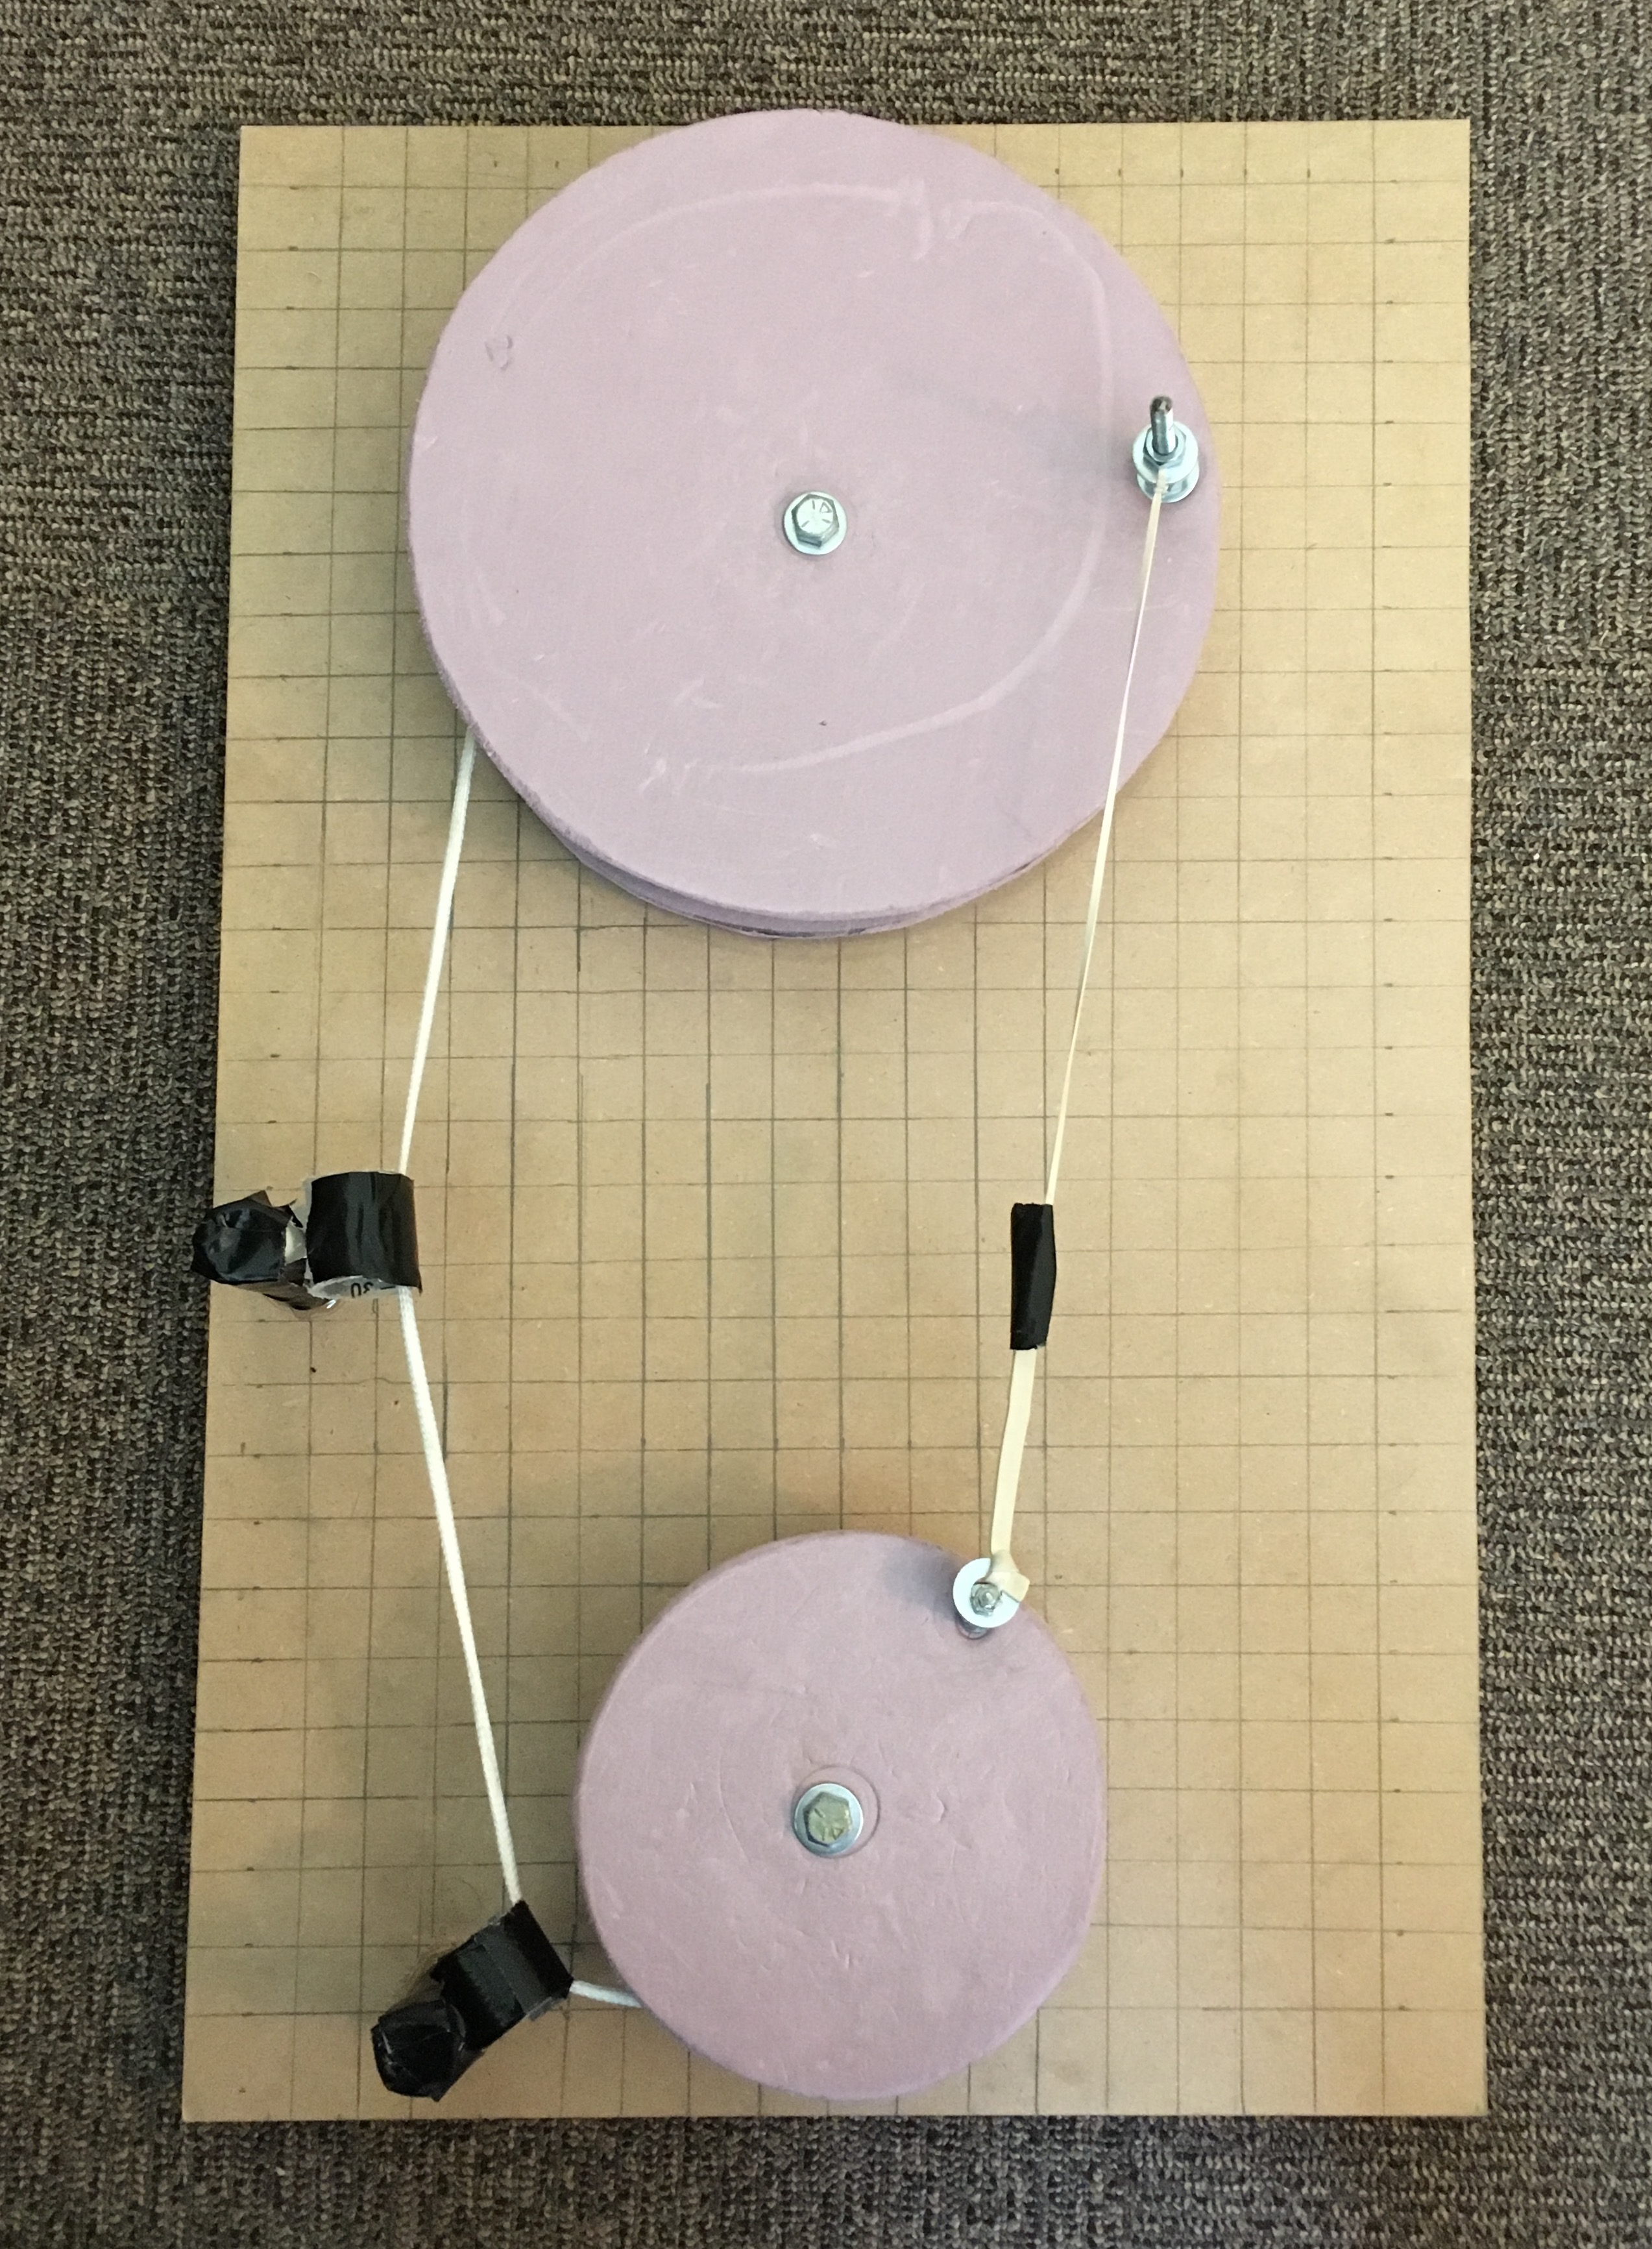
\includegraphics[width=0.35\textwidth]{prototype.jpg}
\end{figure}

%------------------------------------------------

% Describe your prototype and any interesting things about how it was constructed, problems encountered, solutions you invented.
% Include a schematic diagram of the prototype
\section{Prototype}

\begin{figure}[!t]
    \caption{Schematic diagram of the prototype}
    \centering
        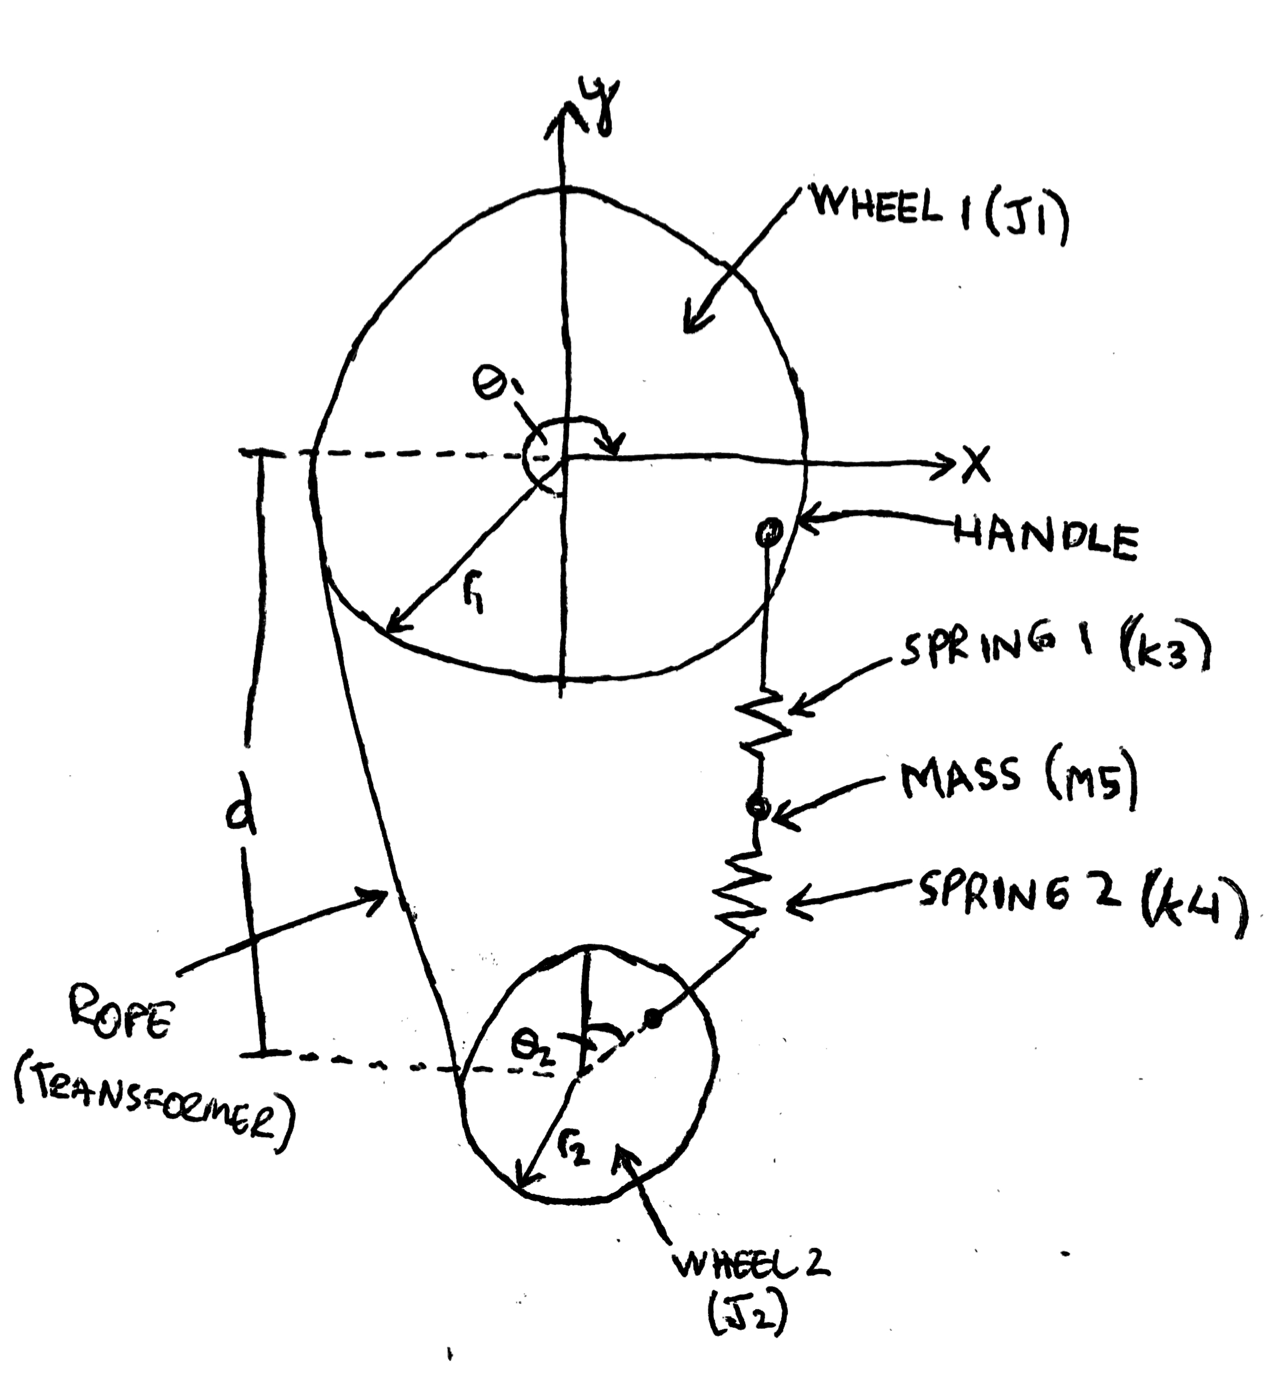
\includegraphics[width=0.35\textwidth]{schematic.png}
\end{figure}

The two rotating wheels are connected through two pathways. Firstly, an inextensible rope which acts as a transformer transfers the angular velocity of the big wheel to the smaller. Secondly, both wheels have fixtures near their edges with are attached to elastics. The two elastics, which vary in length and strength, are connected together with a small mass in the middle. The prototype features mechanical rotation (turning wheels) and translation (moving mass). The wheels are made out of foam and the mass in the middle is a thin screw wrapped in duct tape. A schematic diagram of the prototype can be seen in Figure 2.


The user drives the prototype by rotating the handle of the larger wheel. Both wheels rotate smoothly initially, until the elastic gets stretched far enough to contract rapidly, causing the bottom wheel to slip. When the bottom wheel slips, the rope gains a lot of slack that would often get tangled around the axle. This problem was addressed by adding two guide rails that constrain the rope from tangling. The prototype has to be rewound before every use.


%------------------------------------------------

% Describe your BG, components, constitutive equations, and so on. Explain how you arrived at all the parameters you used. What  measurements did you take? How? Estimations and assumptions made? Theoretical calculations? Extraction of components and separate testing e.g. for springs?
\section{Model}

The bond graph of the prototype can be seen in Figure 3.
\begin{figure}[!h]
    \caption{Bond Graph of the prototype}
    \centering
        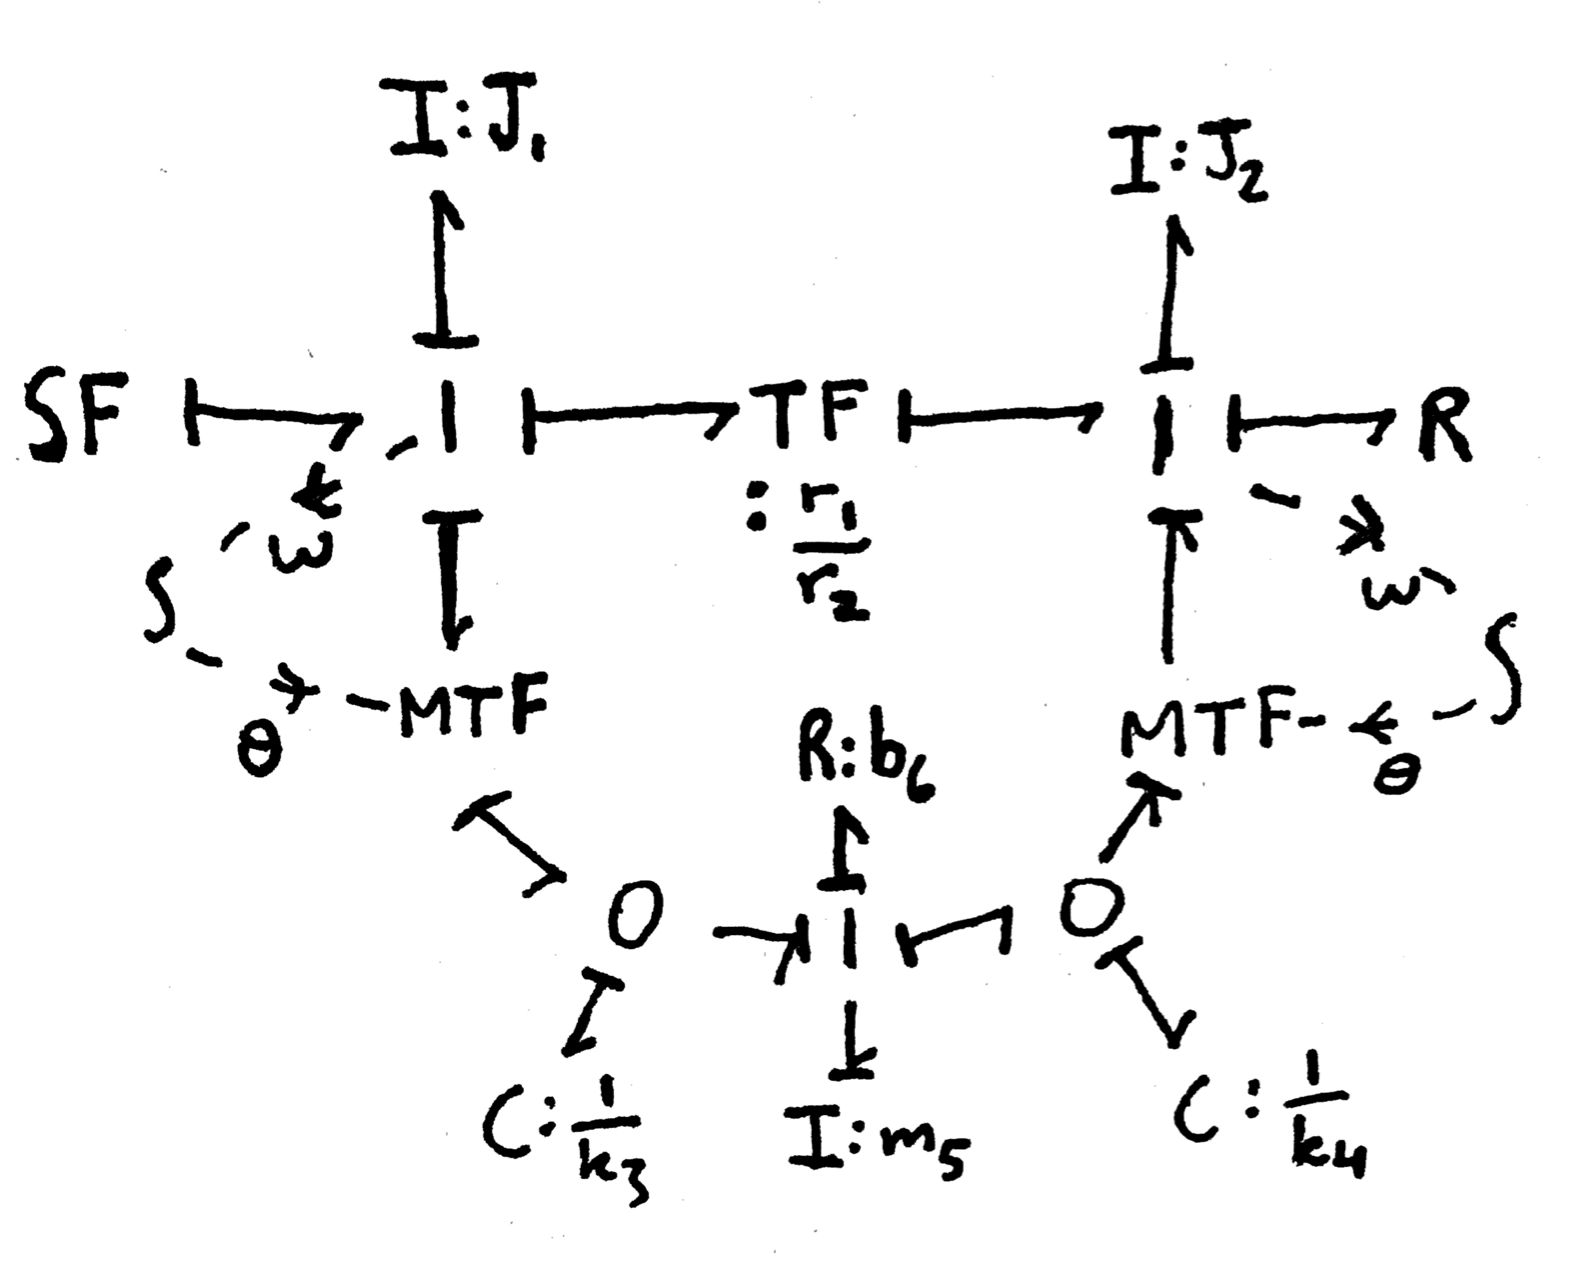
\includegraphics[width=0.3\textwidth]{bg.png}
\end{figure}

The user's input (i.e. turning the big wheel) is considered a source of flow as the user sets the angular velocity. The user will have to change the amount of torque they provide in order to account for the friction of the axle as well as the forces from the elastics. Because both wheels are connected via a taut inextensible rope (i.e. a transformer) and do not slip initially, they are in derivative causality as their angular velocity depends on the user's input velocity. However, when the bottom wheel slips and the rope gains slack, the rope is not taut and no longer acts as a transformer causing the bottom wheel to go into an integral causality state. The R element represents drag friction damping the rotation of the bottom wheel and $b_6$ is the spring damping. Since the prototype requires very precise parameters to work perfectly, the building parameters were chosen simply based on trial and error. The simulations assumes values for parameters, seen in Table 1 of the following section. It is assumed, however, that the springs are both linear.

The modulated transformers represent the fixtures of the elastics on the wheels. As the fixtures move around the edge of the wheels, the distance between them changes, which results in a changing displacement of each elastic. The MTFs depend on $\theta_1$, according the following equations:

\begin{gather*}
x_1 = r_1 \sin(\theta_1) \\
y_1 = r_1 \cos(\theta_1) \\
x_2 = r_2 \sin(\theta_2) = r_2 \sin \left( \frac{r_1}{r_2} \theta_1 \right) \\
y_2 = r_2 \cos(\theta_2) - d = r_2 \cos \left( \frac{r_1}{r_2} \theta_1 \right) - d \\
\end{gather*}

With these positions, the Euclidean distance can be calculated and used in conjunction with the state equations and geometry of the prototype to conduct a MATLAB simulation.

%------------------------------------------------

% What are your state variables and outputs of interest. Give matlab results (plots, not charts of numbers). Do NOT provide massive quantities of outputs. Be very selective and apply engineering acumen. One good output plot may be sufficient. Providing stacks of output plots is not necessary, in fact undesirable and would receive a lower grade. State variables themselves are often not interesting outputs.
\section{Simulation}

The simulation was conducted in three separate stages. The first was the rotation of both wheels through the transfer function of the inextensible rope. The second stage was the slip of the small wheel where the rope gained slack and the wheel moved freely from the force of the elastics. The third stage continues through the rotation of the bigger wheel until the rope is wound tight again and the process can repeat.

\begin{figure}[!h]
    \caption{Simulation (top) vs. Testing (bottom)}
    \centering
        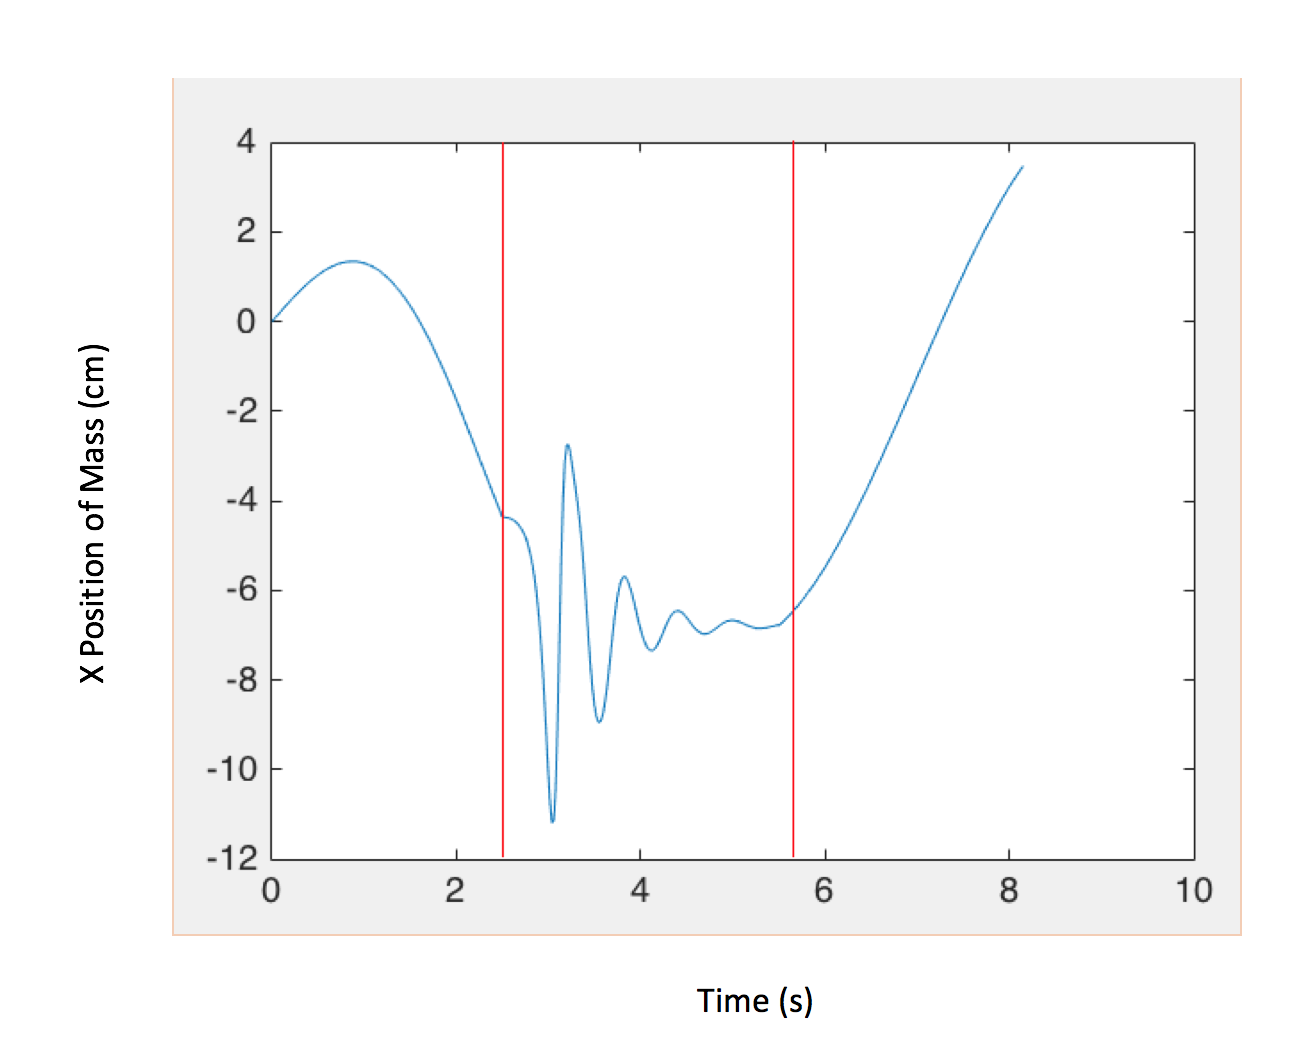
\includegraphics[width=0.45\textwidth]{x.png}
    \centering
        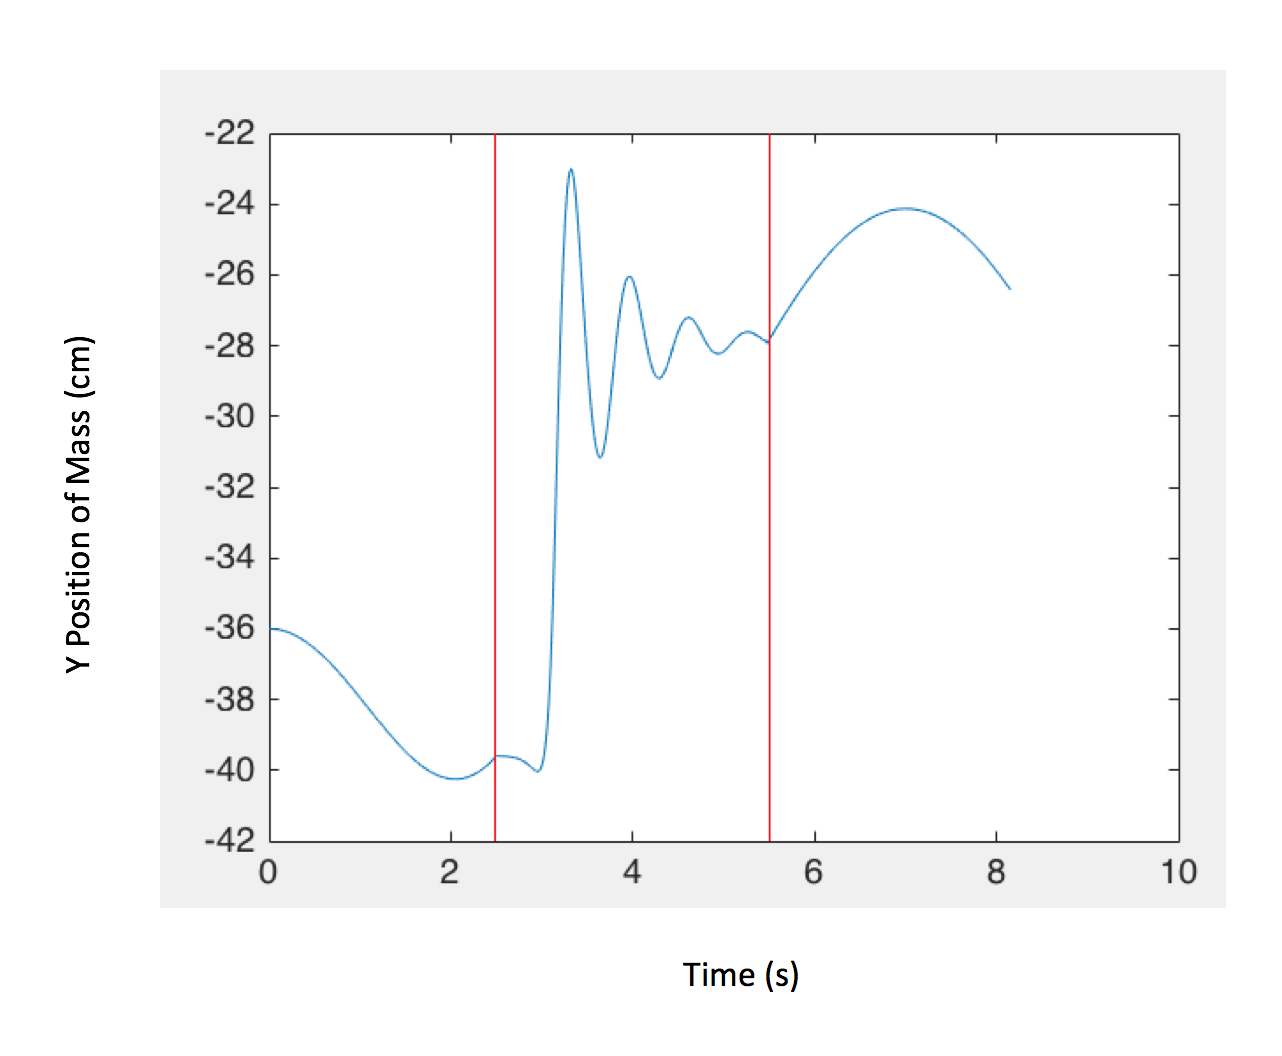
\includegraphics[width=0.45\textwidth]{y.png}
    \centering
        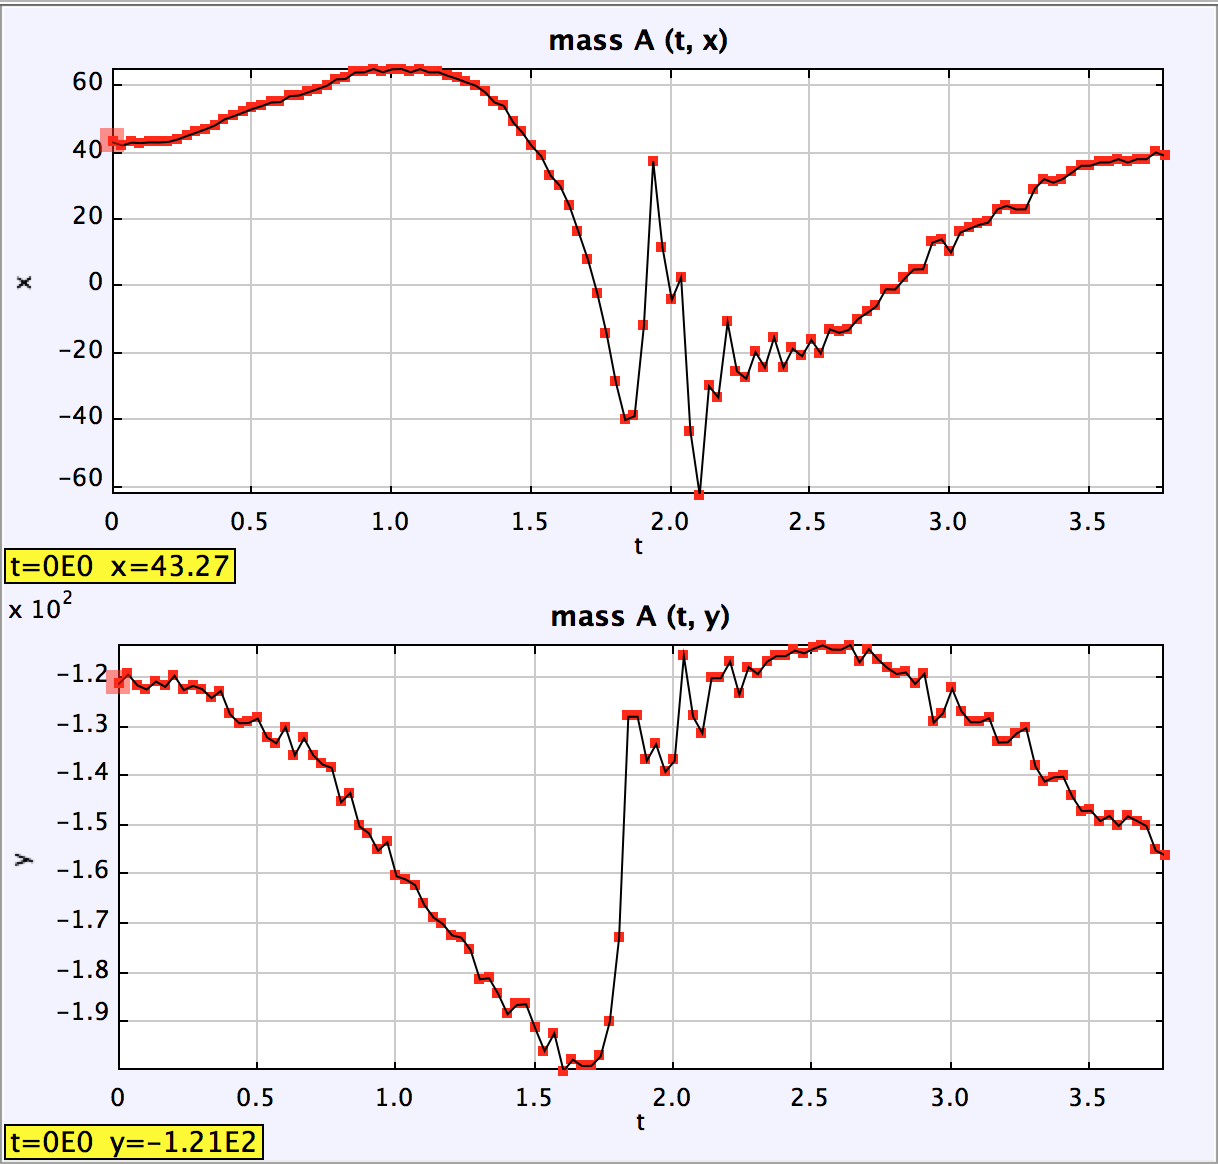
\includegraphics[width=0.45\textwidth]{tracking-plots.png}
\end{figure}

The output of interest is the position of the mass over time. The simulated three stages are shown in the first 2 plots of Figure 4 using red lines as dividers between them. As can be seen, the motion of the mass is first smooth, moving in a sinusoidal fashion until the slip occurs and there begins a damped oscillation. Once the oscillation stops, the big wheel continues to spin moving the mass in a sinusoidal fashion once more.

The simulation was modeled using 4 state variables - the displacement of the two springs ($x_3, x_4$), the momentum of the mass between them ($p_5$) and the angular momentum of the bottom wheel ($L_2$). The values chosen for each of the parameters in the system are shown in Table 1.

\begin{table}
\caption{Parameter values chosen}
\centering
\begin{tabular}{lr}
\toprule
\cmidrule(r){1-2}
Parameter & Value \\
\midrule
$k_3$ & $20$ $N/m$ \\
$k_4$ & $30$ $N/m$ \\
$m_5$ & $0.5$ $kg$ \\
$J_2$ & $25$ $kg \cdot m^2$ \\
$R$ & $125$ $kg \cdot m^2/s$ \\
$b_6$ & $1.5$ $kg/s$ \\
\bottomrule
\end{tabular}
\end{table}

In the first and last stage, all the springs and masses were in static equilibrium at every moment, meaning that the two wheels spun at constant angular velocities and the mass would move according to the applicable geometry. During the slip however, the movement of the bottom wheel due to the applied moment resulted in the bottom spring contracting, creating a disequilibrium. This in turn moves the mass and causes it to oscillate.

%------------------------------------------------

% Compare simulation to data obtained from the system. Describe how well your simulation matches the actual behaviour as determined by an easily observable representative output variable (flashing lights, buzzer, counting rotations, and so on). Could the results be improved? Speculate on any significant descrepancies between test observations and simulation outputs. Explaining your validation process and demonstrating your understanding of the methods are much more important than getting wonderfully close agreement with the behaviour of your prototype.
\section{Discussion}

By comparing the two plots created from the simulation to the ones created from tracking the motion of the mass through software, it can be seen that they are very similar. Firstly, both stages 1 and 3 have similar sinusoidal movements, though the ones from the real model are less smooth and have more chaotic wobbles. This is mostly because of the inconsistency in the source of flow that is the hand moving the top wheel. Moreover, it can be seen that the amplitudes and relative phases of the sinusoidal waves are different. This is because of the inaccurate measurement of the geometries of the wheels. Although measuring the radii of the wheels is trivial, they are not constant as the winding of the rope changes the dimensions of the wheels.

Looking at stage 2 the plots are also very similar, though the oscillation in the simulation is again much smoother and even than the one in the real model. This is mostly because the elastics are not perfectly linear springs and thus do not act like they are modeled in the simulation. However, the oscillations die down at approximately the same rate, meaning the damping was chosen fairly accurately.

\end{document}